% Options for packages loaded elsewhere
\PassOptionsToPackage{unicode}{hyperref}
\PassOptionsToPackage{hyphens}{url}
%
\documentclass[
  ignorenonframetext,
]{beamer}
\usepackage{pgfpages}
\setbeamertemplate{caption}[numbered]
\setbeamertemplate{caption label separator}{: }
\setbeamercolor{caption name}{fg=normal text.fg}
\beamertemplatenavigationsymbolsempty
% Prevent slide breaks in the middle of a paragraph
\widowpenalties 1 10000
\raggedbottom
\setbeamertemplate{part page}{
  \centering
  \begin{beamercolorbox}[sep=16pt,center]{part title}
    \usebeamerfont{part title}\insertpart\par
  \end{beamercolorbox}
}
\setbeamertemplate{section page}{
  \centering
  \begin{beamercolorbox}[sep=12pt,center]{section title}
    \usebeamerfont{section title}\insertsection\par
  \end{beamercolorbox}
}
\setbeamertemplate{subsection page}{
  \centering
  \begin{beamercolorbox}[sep=8pt,center]{subsection title}
    \usebeamerfont{subsection title}\insertsubsection\par
  \end{beamercolorbox}
}
\AtBeginPart{
  \frame{\partpage}
}
\AtBeginSection{
  \ifbibliography
  \else
    \frame{\sectionpage}
  \fi
}
\AtBeginSubsection{
  \frame{\subsectionpage}
}

\usepackage{amsmath,amssymb}
\usepackage{iftex}
\ifPDFTeX
  \usepackage[T1]{fontenc}
  \usepackage[utf8]{inputenc}
  \usepackage{textcomp} % provide euro and other symbols
\else % if luatex or xetex
  \usepackage{unicode-math}
  \defaultfontfeatures{Scale=MatchLowercase}
  \defaultfontfeatures[\rmfamily]{Ligatures=TeX,Scale=1}
\fi
\usepackage{lmodern}
\ifPDFTeX\else  
    % xetex/luatex font selection
\fi
% Use upquote if available, for straight quotes in verbatim environments
\IfFileExists{upquote.sty}{\usepackage{upquote}}{}
\IfFileExists{microtype.sty}{% use microtype if available
  \usepackage[]{microtype}
  \UseMicrotypeSet[protrusion]{basicmath} % disable protrusion for tt fonts
}{}
\makeatletter
\@ifundefined{KOMAClassName}{% if non-KOMA class
  \IfFileExists{parskip.sty}{%
    \usepackage{parskip}
  }{% else
    \setlength{\parindent}{0pt}
    \setlength{\parskip}{6pt plus 2pt minus 1pt}}
}{% if KOMA class
  \KOMAoptions{parskip=half}}
\makeatother
\usepackage{xcolor}
\newif\ifbibliography
\setlength{\emergencystretch}{3em} % prevent overfull lines
\setcounter{secnumdepth}{-\maxdimen} % remove section numbering

\usepackage{color}
\usepackage{fancyvrb}
\newcommand{\VerbBar}{|}
\newcommand{\VERB}{\Verb[commandchars=\\\{\}]}
\DefineVerbatimEnvironment{Highlighting}{Verbatim}{commandchars=\\\{\}}
% Add ',fontsize=\small' for more characters per line
\usepackage{framed}
\definecolor{shadecolor}{RGB}{241,243,245}
\newenvironment{Shaded}{\begin{snugshade}}{\end{snugshade}}
\newcommand{\AlertTok}[1]{\textcolor[rgb]{0.68,0.00,0.00}{#1}}
\newcommand{\AnnotationTok}[1]{\textcolor[rgb]{0.37,0.37,0.37}{#1}}
\newcommand{\AttributeTok}[1]{\textcolor[rgb]{0.40,0.45,0.13}{#1}}
\newcommand{\BaseNTok}[1]{\textcolor[rgb]{0.68,0.00,0.00}{#1}}
\newcommand{\BuiltInTok}[1]{\textcolor[rgb]{0.00,0.23,0.31}{#1}}
\newcommand{\CharTok}[1]{\textcolor[rgb]{0.13,0.47,0.30}{#1}}
\newcommand{\CommentTok}[1]{\textcolor[rgb]{0.37,0.37,0.37}{#1}}
\newcommand{\CommentVarTok}[1]{\textcolor[rgb]{0.37,0.37,0.37}{\textit{#1}}}
\newcommand{\ConstantTok}[1]{\textcolor[rgb]{0.56,0.35,0.01}{#1}}
\newcommand{\ControlFlowTok}[1]{\textcolor[rgb]{0.00,0.23,0.31}{\textbf{#1}}}
\newcommand{\DataTypeTok}[1]{\textcolor[rgb]{0.68,0.00,0.00}{#1}}
\newcommand{\DecValTok}[1]{\textcolor[rgb]{0.68,0.00,0.00}{#1}}
\newcommand{\DocumentationTok}[1]{\textcolor[rgb]{0.37,0.37,0.37}{\textit{#1}}}
\newcommand{\ErrorTok}[1]{\textcolor[rgb]{0.68,0.00,0.00}{#1}}
\newcommand{\ExtensionTok}[1]{\textcolor[rgb]{0.00,0.23,0.31}{#1}}
\newcommand{\FloatTok}[1]{\textcolor[rgb]{0.68,0.00,0.00}{#1}}
\newcommand{\FunctionTok}[1]{\textcolor[rgb]{0.28,0.35,0.67}{#1}}
\newcommand{\ImportTok}[1]{\textcolor[rgb]{0.00,0.46,0.62}{#1}}
\newcommand{\InformationTok}[1]{\textcolor[rgb]{0.37,0.37,0.37}{#1}}
\newcommand{\KeywordTok}[1]{\textcolor[rgb]{0.00,0.23,0.31}{\textbf{#1}}}
\newcommand{\NormalTok}[1]{\textcolor[rgb]{0.00,0.23,0.31}{#1}}
\newcommand{\OperatorTok}[1]{\textcolor[rgb]{0.37,0.37,0.37}{#1}}
\newcommand{\OtherTok}[1]{\textcolor[rgb]{0.00,0.23,0.31}{#1}}
\newcommand{\PreprocessorTok}[1]{\textcolor[rgb]{0.68,0.00,0.00}{#1}}
\newcommand{\RegionMarkerTok}[1]{\textcolor[rgb]{0.00,0.23,0.31}{#1}}
\newcommand{\SpecialCharTok}[1]{\textcolor[rgb]{0.37,0.37,0.37}{#1}}
\newcommand{\SpecialStringTok}[1]{\textcolor[rgb]{0.13,0.47,0.30}{#1}}
\newcommand{\StringTok}[1]{\textcolor[rgb]{0.13,0.47,0.30}{#1}}
\newcommand{\VariableTok}[1]{\textcolor[rgb]{0.07,0.07,0.07}{#1}}
\newcommand{\VerbatimStringTok}[1]{\textcolor[rgb]{0.13,0.47,0.30}{#1}}
\newcommand{\WarningTok}[1]{\textcolor[rgb]{0.37,0.37,0.37}{\textit{#1}}}

\providecommand{\tightlist}{%
  \setlength{\itemsep}{0pt}\setlength{\parskip}{0pt}}\usepackage{longtable,booktabs,array}
\usepackage{calc} % for calculating minipage widths
\usepackage{caption}
% Make caption package work with longtable
\makeatletter
\def\fnum@table{\tablename~\thetable}
\makeatother
\usepackage{graphicx}
\makeatletter
\newsavebox\pandoc@box
\newcommand*\pandocbounded[1]{% scales image to fit in text height/width
  \sbox\pandoc@box{#1}%
  \Gscale@div\@tempa{\textheight}{\dimexpr\ht\pandoc@box+\dp\pandoc@box\relax}%
  \Gscale@div\@tempb{\linewidth}{\wd\pandoc@box}%
  \ifdim\@tempb\p@<\@tempa\p@\let\@tempa\@tempb\fi% select the smaller of both
  \ifdim\@tempa\p@<\p@\scalebox{\@tempa}{\usebox\pandoc@box}%
  \else\usebox{\pandoc@box}%
  \fi%
}
% Set default figure placement to htbp
\def\fps@figure{htbp}
\makeatother

\usepackage{adjustbox}
\usepackage{geometry}
\geometry{margin=1cm}
\AtBeginEnvironment{verbatim}{\footnotesize}
\makeatletter
\@ifpackageloaded{caption}{}{\usepackage{caption}}
\AtBeginDocument{%
\ifdefined\contentsname
  \renewcommand*\contentsname{Table of contents}
\else
  \newcommand\contentsname{Table of contents}
\fi
\ifdefined\listfigurename
  \renewcommand*\listfigurename{List of Figures}
\else
  \newcommand\listfigurename{List of Figures}
\fi
\ifdefined\listtablename
  \renewcommand*\listtablename{List of Tables}
\else
  \newcommand\listtablename{List of Tables}
\fi
\ifdefined\figurename
  \renewcommand*\figurename{Figure}
\else
  \newcommand\figurename{Figure}
\fi
\ifdefined\tablename
  \renewcommand*\tablename{Table}
\else
  \newcommand\tablename{Table}
\fi
}
\@ifpackageloaded{float}{}{\usepackage{float}}
\floatstyle{ruled}
\@ifundefined{c@chapter}{\newfloat{codelisting}{h}{lop}}{\newfloat{codelisting}{h}{lop}[chapter]}
\floatname{codelisting}{Listing}
\newcommand*\listoflistings{\listof{codelisting}{List of Listings}}
\makeatother
\makeatletter
\makeatother
\makeatletter
\@ifpackageloaded{caption}{}{\usepackage{caption}}
\@ifpackageloaded{subcaption}{}{\usepackage{subcaption}}
\makeatother

\usepackage{bookmark}

\IfFileExists{xurl.sty}{\usepackage{xurl}}{} % add URL line breaks if available
\urlstyle{same} % disable monospaced font for URLs
\hypersetup{
  pdftitle={Group Challenge},
  pdfauthor={Jia Guo, Mattias Blum, Jinxiang Ma, Noah Kochanski},
  hidelinks,
  pdfcreator={LaTeX via pandoc}}


\title{Group Challenge}
\author{Jia Guo, Mattias Blum, Jinxiang Ma, Noah Kochanski}
\date{}

\begin{document}
\frame{\titlepage}


\section{Group Challenge 1}\label{group-challenge-1}

\begin{frame}{DHS}
\phantomsection\label{dhs}
Our data comes from the \href{https://dhsprogram.com}{Demographic Health
Survey Program}.

\begin{itemize}
\tightlist
\item
  The Demographic Health Survey (DHS) is a national level survey
  conducted in many countries around the globe.
\item
  DHS collects and distributes a plethora of data on aspects of
  developing nations.
\end{itemize}
\end{frame}

\begin{frame}{DHS}
\phantomsection\label{dhs-1}
\begin{itemize}
\item
  Our particular analysis will be conducted on the \textbf{birth}
  related survey from 2017-2018 in Bangladesh.
\item
  For this survey, households were sampled in particular clusters
  (villages or town centers) around the country.
\item
  If a mother was surveyed in a particular cluster location, they were
  asked if they had any children under the age of \textbf{5}. If they
  did, then a particular question was about their children under the age
  of 5.
\item
  For this particular survey, 2383 observations (births) were recorded
  across Bangladesh.
\end{itemize}
\end{frame}

\begin{frame}{Analysis of Covariates - Summary of Main Dataset and
Cluster Metadata}
\phantomsection\label{analysis-of-covariates---summary-of-main-dataset-and-cluster-metadata}
The main dataset contains 29 covariates. One of these covariates is
cluster\_id, a unique numeric key identifying a site of measurement.
Another dataset contains metadata pertaining to each individual cluster,
detailing:

\begin{itemize}
\item
  Geographic location (latitude, longitude)
\item
  ID for the DHS survey
\item
  Year of the survey
\item
  Coordinate reference system (CRS: WGS84)
\end{itemize}
\end{frame}

\begin{frame}{Analysis of Covariates - Summary of Main Dataset and
Cluster Metadata}
\phantomsection\label{analysis-of-covariates---summary-of-main-dataset-and-cluster-metadata-1}
Although none of the metadata fields will be used for analysis, we must
join on cluster\_id to recover geographic locations.
\end{frame}

\begin{frame}{Household and Demographic Variables}
\phantomsection\label{household-and-demographic-variables}
\begin{itemize}
\tightlist
\item
  Cluster ID from DHS data\\
\item
  Household number within the cluster\\
\item
  Rank of individual within household\\
\item
  Number of household members\\
\item
  Number of children under 5 in household\\
\item
  Gender of household head
\end{itemize}
\end{frame}

\begin{frame}{Household and Demographic Variables}
\phantomsection\label{household-and-demographic-variables-1}
\begin{itemize}
\tightlist
\item
  Urban or rural residence\\
\item
  Wealth index category\\
\item
  Survey weighting variable\\
\item
  Stratification variable for survey design\\
\item
  PSU identifier for survey design
\end{itemize}
\end{frame}

\begin{frame}{Maternal Variables}
\phantomsection\label{maternal-variables}
\begin{itemize}
\tightlist
\item
  Age of the mother\\
\item
  Education level of the mother\\
\item
  Occupation type\\
\item
  Mother's height (cm)\\
\item
  Mother's BMI\\
\item
  Marital status of the mother\\
\item
  Number of antenatal visits attended\\
\item
  Diagnosed with high blood pressure\\
\item
  Diagnosed with diabetes
\end{itemize}
\end{frame}

\begin{frame}{Child Variables}
\phantomsection\label{child-variables}
\begin{itemize}
\tightlist
\item
  Birth order of the child\\
\item
  Sex of child\\
\item
  Source of birth weight measurement\\
\item
  Birth weight in grams\\
\item
  Categorized birth weight\\
\item
  Date of birth
\end{itemize}
\end{frame}

\begin{frame}{Household Infrastructure Variables}
\phantomsection\label{household-infrastructure-variables}
\begin{itemize}
\tightlist
\item
  Type of drinking water source\\
\item
  Type of toilet facility\\
\item
  Availability of electricity\\
\item
  Floor material\\
\item
  Type of cooking fuel
\end{itemize}
\end{frame}

\begin{frame}{Analysis of Covariates - Pairwise Correlation of Numeric
Variables}
\phantomsection\label{analysis-of-covariates---pairwise-correlation-of-numeric-variables}
\pandocbounded{\includegraphics[keepaspectratio]{gc_files/figure-beamer/unnamed-chunk-4-1.pdf}}
\end{frame}

\begin{frame}[fragile]{Analysis of Covariates - Variance Inflation
Factor}
\phantomsection\label{analysis-of-covariates---variance-inflation-factor}
\begin{verbatim}
        household_rank     mother_current_age        household_water 
              2.555389               1.983368               1.009798 
     household_members      household_under_5 household_cooking_fuel 
              2.615649               1.213228               1.747282 
         mother_height             mother_bmi           wealth_index 
              1.069034               1.248646               1.765605 
           birth_order       antenatal_visits           birth_weight 
              2.011993               1.090437               1.030285 
         survey_weight                 strata  primary_sampling_unit 
              1.552240              31.586843              32.943293 
\end{verbatim}
\end{frame}

\begin{frame}{Analysis of Covariates - Autocorrelation}
\phantomsection\label{analysis-of-covariates---autocorrelation}
\pandocbounded{\includegraphics[keepaspectratio]{gc_files/figure-beamer/unnamed-chunk-6-1.pdf}}
\end{frame}

\begin{frame}[fragile]{Spatial Domain}
\phantomsection\label{spatial-domain}
\begin{itemize}
\tightlist
\item
  The study covers \textbf{Bangladesh}, with observations from
  \textbf{2,383 participants} distributed across geographic coordinates
  (latitude and longitude).\\
\item
  Each participant's location was masked by assigning them to a
  \textbf{cluster centroid} (via \texttt{clusterid}).\\
\item
  To create pseudo-unique locations, small \textbf{i.i.d. Gaussian
  noise} (SD = 0.001 degrees) was added to latitude/longitude.\\
\item
  Observations are \textbf{spatially indexed} using these randomized
  coordinates.
\end{itemize}
\end{frame}

\begin{frame}{Spatial Dependence}
\phantomsection\label{spatial-dependence}
\begin{itemize}
\tightlist
\item
  \textbf{Covariance decay with distance} is a reasonable assumption due
  to spatial dependence of birth weight on environmental factors (e.g.,
  local temperature).\\
\item
  \textbf{Spatial correlation} may arise from:

  \begin{itemize}
  \tightlist
  \item
    Shared environmental exposures (e.g., regional climate,
    pollution).\\
  \item
    Socioeconomic conditions that vary geographically.\\
  \end{itemize}
\item
  Using \textbf{distance-based covariance} assumes that \textbf{mothers
  in close proximity experience similar environmental influences}
  affecting birth outcomes.
\end{itemize}
\end{frame}

\begin{frame}{Empirical Variogram}
\phantomsection\label{empirical-variogram}
\pandocbounded{\includegraphics[keepaspectratio]{gc_files/figure-beamer/unnamed-chunk-7-1.pdf}}
\end{frame}

\begin{frame}{Empirical Variogram}
\phantomsection\label{empirical-variogram-1}
The empirical variogram for birth weight displays three key features:

\begin{enumerate}
\tightlist
\item
  A decrease in semivariance at very short distances (\textless20 km),
  likely reflecting the artificial noise added to cluster centroids.
  This ``dip'' represents reduced variability within clusters due to the
  imposed randomization, as participants from the same original cluster
  are now treated as spatially distinct but still share similar
  environmental conditions.
\end{enumerate}
\end{frame}

\begin{frame}{Empirical Variogram}
\phantomsection\label{empirical-variogram-2}
\begin{enumerate}
\setcounter{enumi}{1}
\item
  An increasing trend between 20--80 km, indicating spatial dependence.
  Rising semivariance with distance suggests that birth weights become
  less similar as geographic separation increases, consistent with
  spatial autocorrelation.
\item
  A plateau beyond 80 km, implying the spatial correlation range (where
  covariance stabilizes) is reached.
\end{enumerate}
\end{frame}

\begin{frame}{Empirical Variogram}
\phantomsection\label{empirical-variogram-3}
Overall, the spatial pattern aligns with the hypothesis that
environmental factors like temperature---which vary regionally---may
contribute to geographic disparities in birth weight. Further
investigation into the covariance structure and model diagnostics would
strengthen these conclusions.
\end{frame}

\begin{frame}{Cluster Locations}
\phantomsection\label{cluster-locations}
\pandocbounded{\includegraphics[keepaspectratio]{gc_files/figure-beamer/unnamed-chunk-10-1.pdf}}
\end{frame}

\begin{frame}{Wealth Index}
\phantomsection\label{wealth-index}
\pandocbounded{\includegraphics[keepaspectratio]{gc_files/figure-beamer/unnamed-chunk-12-1.pdf}}
\end{frame}

\begin{frame}{Wealth Index}
\phantomsection\label{wealth-index-1}
The data shows both large-scale trends (visible in heat maps) and local
variation Urban-rural differences create discontinuities in the spatial
pattern River systems in Bangladesh might create natural
boundaries/corridors for spatial correlation The jittering adds some
noise to the spatial relationships but shouldn't significantly affect
large-scale patterns
\end{frame}

\begin{frame}{Birth Weight}
\phantomsection\label{birth-weight}
\pandocbounded{\includegraphics[keepaspectratio]{gc_files/figure-beamer/unnamed-chunk-13-1.pdf}}
\end{frame}

\begin{frame}{Maternal Education}
\phantomsection\label{maternal-education}
\pandocbounded{\includegraphics[keepaspectratio]{gc_files/figure-beamer/unnamed-chunk-14-1.pdf}}
\end{frame}

\begin{frame}{Household Water Access}
\phantomsection\label{household-water-access}
\pandocbounded{\includegraphics[keepaspectratio]{gc_files/figure-beamer/unnamed-chunk-15-1.pdf}}
\end{frame}

\begin{frame}{Residence Type and Birth Weight}
\phantomsection\label{residence-type-and-birth-weight}
\pandocbounded{\includegraphics[keepaspectratio]{gc_files/figure-beamer/unnamed-chunk-16-1.pdf}}
\end{frame}

\begin{frame}{Possible Research Questions}
\phantomsection\label{possible-research-questions}
How do birth weights vary between urban and rural areas in Bangladesh?
Is there a relationship between household wealth and birth weight
outcomes? Do regions with better water access show improved birth weight
outcomes? How does mother's education level correlate with birth weight
across different regions?
\end{frame}

\begin{frame}{Possible Research Questions}
\phantomsection\label{possible-research-questions-1}
Are there distinct regional clusters of high/low birth weights? Do
coastal regions show different patterns compared to inland areas? Is
there evidence of spillover effects from urban centers to surrounding
rural areas? How do major river systems influence the spatial
distribution of birth weights?
\end{frame}

\begin{frame}{Possible Research Questions}
\phantomsection\label{possible-research-questions-2}
How strongly does wealth index predict birth weight when controlling for
spatial correlation? Is the relationship between mother's education and
birth weight consistent across regions? Do areas with better
infrastructure (water access, healthcare facilities) show more
consistent birth weights
\end{frame}

\begin{frame}{References}
\phantomsection\label{references}
National Institute of Population Research and Training (NIPORT), and
ICF. (2020).~\emph{Bangladesh Demographic and Health Survey 2017-18}.
Dhaka, Bangladesh, and Rockville, Maryland, USA: NIPORT and ICF.
\end{frame}

\section{Group Challenge 2}\label{group-challenge-2}

\begin{frame}[fragile]{Loading Data}
\phantomsection\label{loading-data}
\begin{Shaded}
\begin{Highlighting}[]
\NormalTok{birth\_imp }\OtherTok{\textless{}{-}} \FunctionTok{readRDS}\NormalTok{(}\StringTok{\textquotesingle{}data/input/birth\_imp.RDS\textquotesingle{}}\NormalTok{) }\CommentTok{\# Load the imputed birth data}
\NormalTok{cluster\_locations }\OtherTok{\textless{}{-}} \FunctionTok{read\_csv}\NormalTok{(}\StringTok{\textquotesingle{}data/input/cluster\_locations.csv\textquotesingle{}}\NormalTok{) }\SpecialCharTok{\%\textgreater{}\%} 
  \FunctionTok{rename}\NormalTok{(}\AttributeTok{clusterid =}\NormalTok{ DHSCLUST) }\SpecialCharTok{\%\textgreater{}\%} 
  \FunctionTok{select}\NormalTok{(clusterid, LATNUM, LONGNUM)}
\NormalTok{reg\_data }\OtherTok{\textless{}{-}} \FunctionTok{left\_join}\NormalTok{(birth\_imp, cluster\_locations)}
\end{Highlighting}
\end{Shaded}

The dataset birth\_imp.RDS contains birth-related data. Another dataset,
cluster\_locations.csv, contains spatial information about clusters,
including latitude (LATNUM) and longitude (LONGNUM). The column DHSCLUST
is renamed to clusterid to maintain consistency across datasets, and
only relevant columns are selected.

The two datasets are merged using left\_join(), ensuring that
birth-related records are matched with their corresponding cluster
locations based on the clusterid field.
\end{frame}

\begin{frame}[fragile]{Standard Linear Regression}
\phantomsection\label{standard-linear-regression}
\begin{verbatim}

Call:
lm(formula = birth_weight ~ birth_weight_type + mother_bmi + 
    sex_of_child + mother_current_age, data = reg_data)

Residuals:
    Min      1Q  Median      3Q     Max 
-2342.4  -457.1    12.6   467.6  3239.3 

Coefficients:
                                Estimate Std. Error t value Pr(>|t|)    
(Intercept)                   2653.29795   90.88762  29.193  < 2e-16 ***
birth_weight_typewritten card  -89.92422   71.37700  -1.260 0.207848    
mother_bmi                       0.16857    0.03512   4.800 1.69e-06 ***
sex_of_childmale               106.70534   28.71063   3.717 0.000207 ***
mother_current_age              -4.52190    2.74553  -1.647 0.099689 .  
---
Signif. codes:  0 '***' 0.001 '**' 0.01 '*' 0.05 '.' 0.1 ' ' 1

Residual standard error: 698.4 on 2378 degrees of freedom
Multiple R-squared:  0.01605,   Adjusted R-squared:  0.01439 
F-statistic: 9.695 on 4 and 2378 DF,  p-value: 8.905e-08
\end{verbatim}
\end{frame}

\begin{frame}{Standard Linear Regression}
\phantomsection\label{standard-linear-regression-1}
The linear regression model explains a small portion of the variance in
birth weight, with a coefficient of determination of 0.016, indicating
that the included predictors only account for about 1.6\% of the
variation. The low coefficient of determination suggests that additional
factors, possibly spatial or environmental variables, may be influencing
birth weight.

The intercept, 2653 grams, represents the estimated birth weight for a
female child, with an unspecified birth weight type, and at average
maternal BMI and age. Mother BMI has a significant positive effect on
birth weight, 0.17 grams per unit increase, suggesting that higher BMI
is associated with heavier newborns.

Male children weigh about 107 grams more than females on average. The
effect of mother age is negative, 4.52 grams decrease per year, but not
statistically significant at the 5\% level, implying weak evidence for
an age-related decline in birth weight.

The variable birth weight type (written card vs.~mother recall) has an
estimated difference of -90 grams but is not statistically significant,
indicating no strong evidence that recorded birth weight type impacts
the outcome.
\end{frame}

\begin{frame}{Residual Visualization}
\phantomsection\label{residual-visualization}
\pandocbounded{\includegraphics[keepaspectratio]{gc_files/figure-beamer/unnamed-chunk-19-1.pdf}}
\end{frame}

\begin{frame}{Residual Visualization}
\phantomsection\label{residual-visualization-1}
This scatter plot visualizes the residuals from the linear regression
model across spatial coordinates (LATNUM and LONGNUM). Each point
represents a geographic location, and the color gradient indicates the
magnitude of the residuals. Yellow/Green regions represent positive
residuals, where the model underestimates birth weight. Blue/Purple
regions represent negative residuals, where the model overestimates
birth weight. Near-zero residuals (mid-range colors) indicate areas
where the model's predictions are more accurate. Base on this scatter
plot, clusters of similar residual values (e.g., regions where residuals
are predominantly positive or negative) suggest that there is a spatial
correlation in the errors. This indicates that the linear model may not
fully account for spatial dependencies in the data.
\end{frame}

\begin{frame}{Empirical Variogram}
\phantomsection\label{empirical-variogram-4}
\pandocbounded{\includegraphics[keepaspectratio]{gc_files/figure-beamer/unnamed-chunk-20-1.pdf}}
\end{frame}

\begin{frame}{Empirical Variogram}
\phantomsection\label{empirical-variogram-5}
The empirical variogram of residuals reveals the spatial dependence
structure of unexplained variation after fitting the linear model. The
increasing trend in semivariance at short distances (within 50
kilometers) suggests positive spatial autocorrelation, indicating that
residuals from nearby locations tend to be similar. The lack of a clear
sill suggests that spatial dependence persists beyond the observed range
or that non-stationarity may be present. Fluctuations in the variogram
could be due to noise, uneven spatial sampling, or anisotropy in the
spatial process.
\end{frame}

\begin{frame}[fragile]{Bayesian Regression}
\phantomsection\label{bayesian-regression}
\begin{block}{Preparing Data}
\phantomsection\label{preparing-data}
\begin{Shaded}
\begin{Highlighting}[]
\NormalTok{X }\OtherTok{\textless{}{-}}\NormalTok{ reg\_data }\SpecialCharTok{\%\textgreater{}\%} \FunctionTok{select}\NormalTok{(birth\_weight\_type, mother\_bmi, sex\_of\_child, mother\_current\_age) }\SpecialCharTok{\%\textgreater{}\%} \FunctionTok{as.matrix}\NormalTok{()}
\NormalTok{y }\OtherTok{\textless{}{-}}\NormalTok{ reg\_data }\SpecialCharTok{\%\textgreater{}\%} \FunctionTok{select}\NormalTok{(birth\_weight) }\SpecialCharTok{\%\textgreater{}\%} \FunctionTok{as.matrix}\NormalTok{()}
\NormalTok{p }\OtherTok{\textless{}{-}} \FunctionTok{ncol}\NormalTok{(X)}
\NormalTok{n }\OtherTok{\textless{}{-}} \FunctionTok{nrow}\NormalTok{(X)}
\end{Highlighting}
\end{Shaded}

The predictor variables are extracted into a matrix X, while the
response variable birth\_weight is stored in a separate matrix y. The
number of predictors is assigned to p, and the total number of
observations is stored in n.
\end{block}

\begin{block}{Add Random Noise to Coordinates}
\phantomsection\label{add-random-noise-to-coordinates}
\begin{Shaded}
\begin{Highlighting}[]
\NormalTok{coords }\OtherTok{\textless{}{-}}\NormalTok{ cluster\_locations }\SpecialCharTok{\%\textgreater{}\%} \FunctionTok{select}\NormalTok{(LATNUM, LONGNUM) }
\NormalTok{coords }\OtherTok{\textless{}{-}}\NormalTok{ coords }\SpecialCharTok{+} \FunctionTok{rnorm}\NormalTok{(}\AttributeTok{n =}\NormalTok{ p}\SpecialCharTok{*}\NormalTok{n)}
\end{Highlighting}
\end{Shaded}

Random noise is added to the coordinates of each cluster. This slight
perturbation ensures that spatial locations are not exactly identical
\end{block}
\end{frame}

\begin{frame}[fragile]{Bayesian Regression}
\phantomsection\label{bayesian-regression-1}
\begin{block}{Intialize MCMC}
\phantomsection\label{intialize-mcmc}
\begin{Shaded}
\begin{Highlighting}[]
\NormalTok{n.samples }\OtherTok{\textless{}{-}} \DecValTok{2000} \CommentTok{\# Number of MCMC iterations}
\NormalTok{starting }\OtherTok{\textless{}{-}} \FunctionTok{list}\NormalTok{(}\StringTok{"phi"}\OtherTok{=}\DecValTok{3}\SpecialCharTok{/}\FloatTok{0.5}\NormalTok{, }\StringTok{"sigma.sq"}\OtherTok{=}\DecValTok{50}\NormalTok{, }\StringTok{"tau.sq"}\OtherTok{=}\DecValTok{1}\NormalTok{) }\CommentTok{\# Inital Value for MCMC}
\NormalTok{tuning }\OtherTok{\textless{}{-}} \FunctionTok{list}\NormalTok{(}\StringTok{"phi"}\OtherTok{=}\FloatTok{0.1}\NormalTok{, }\StringTok{"sigma.sq"}\OtherTok{=}\FloatTok{0.1}\NormalTok{, }\StringTok{"tau.sq"}\OtherTok{=}\FloatTok{0.1}\NormalTok{) }\CommentTok{\# Defining Tuning Parameters}
\end{Highlighting}
\end{Shaded}

The number of samples for the Markov Chain Monte Carlo (MCMC) process is
set to 2000. This controls how many iterations the Bayesian inference
process will perform to estimate spatial relationships. For initial
values, the parameter phi controls the range of spatial correlation,
sigma.sq represents the variance of the spatial process, and tau.sq
captures small-scale variability or measurement noise. Tuning parameters
determine the step sizes used in the MCMC algorithm. Proper tuning
ensures efficient sampling and improves convergence.
\end{block}
\end{frame}

\begin{frame}[fragile]{Bayesian Regression}
\phantomsection\label{bayesian-regression-2}
\begin{block}{Prior Distribution \& Covariance model}
\phantomsection\label{prior-distribution-covariance-model}
\begin{Shaded}
\begin{Highlighting}[]
\NormalTok{priors}\FloatTok{.1} \OtherTok{\textless{}{-}} \FunctionTok{list}\NormalTok{(}\StringTok{"beta.Norm"}\OtherTok{=}\FunctionTok{list}\NormalTok{(}\FunctionTok{rep}\NormalTok{(}\DecValTok{0}\NormalTok{,p), }\FunctionTok{diag}\NormalTok{(}\DecValTok{1000}\NormalTok{,p)),}
                 \StringTok{"phi.Unif"}\OtherTok{=}\FunctionTok{c}\NormalTok{(}\FloatTok{0.1}\NormalTok{, }\DecValTok{3}\SpecialCharTok{/}\FloatTok{0.1}\NormalTok{), }
                 \StringTok{"sigma.sq.IG"}\OtherTok{=}\FunctionTok{c}\NormalTok{(}\DecValTok{2}\NormalTok{, }\DecValTok{2}\NormalTok{),}
                 \StringTok{"tau.sq.IG"}\OtherTok{=}\FunctionTok{c}\NormalTok{(}\DecValTok{2}\NormalTok{, }\FloatTok{0.1}\NormalTok{))}
\NormalTok{cov.model }\OtherTok{\textless{}{-}} \StringTok{"exponential"}                 
\end{Highlighting}
\end{Shaded}

Prior distributions are assigned to model parameters. The regression
coefficients (beta.Norm) follow a normal distribution centered at zero
with high variance. The spatial range parameter (phi) has a uniform
prior. The variances (sigma.sq and tau.sq) follow inverse-gamma
distributions, ensuring positive values while allowing flexibility.

The covariance structure is set to an exponential model, where spatial
correlation decays exponentially with distance. This choice assumes that
nearby locations are more strongly correlated than distant ones.
\end{block}
\end{frame}

\begin{frame}[fragile]{Bayesian Regression}
\phantomsection\label{bayesian-regression-3}
\begin{Shaded}
\begin{Highlighting}[]
\NormalTok{n.report }\OtherTok{\textless{}{-}} \DecValTok{500}
\NormalTok{verbose }\OtherTok{\textless{}{-}} \ConstantTok{TRUE}

\NormalTok{m}\FloatTok{.1} \OtherTok{\textless{}{-}} \FunctionTok{spLM}\NormalTok{(y}\SpecialCharTok{\textasciitilde{}}\NormalTok{X, }\AttributeTok{coords=}\FunctionTok{as.matrix}\NormalTok{(coords), }\AttributeTok{starting=}\NormalTok{starting,}
           \AttributeTok{tuning=}\NormalTok{tuning, }\AttributeTok{priors=}\NormalTok{priors}\FloatTok{.1}\NormalTok{, }\AttributeTok{cov.model=}\NormalTok{cov.model,}
           \AttributeTok{n.samples=}\NormalTok{n.samples, }\AttributeTok{verbose=}\NormalTok{verbose, }\AttributeTok{n.report=}\NormalTok{n.report)}

\FunctionTok{summary}\NormalTok{(m}\FloatTok{.1}\SpecialCharTok{$}\NormalTok{p.theta.samples) }\CommentTok{\#Summarize Posterior Distribution}
\end{Highlighting}
\end{Shaded}

\begin{verbatim}

Iterations = 1:5000
Thinning interval = 1 
Number of chains = 1 
Sample size per chain = 5000 

1. Empirical mean and standard deviation for each variable,
   plus standard error of the mean:

              Mean        SD  Naive SE Time-series SE
sigma.sq 7.543e+05 9.280e+04 1.312e+03      1.418e+04
tau.sq   6.797e-02 8.232e-02 1.164e-03      9.566e-03
phi      2.963e+01 1.539e+00 2.177e-02      2.414e-01

2. Quantiles for each variable:

              2.5%       25%       50%       75%     97.5%
sigma.sq 7.113e+05 7.492e+05 7.652e+05 7.770e+05 8.156e+05
tau.sq   2.384e-02 3.920e-02 5.048e-02 6.893e-02 1.926e-01
phi      2.651e+01 2.978e+01 2.992e+01 2.995e+01 2.998e+01
\end{verbatim}
\end{frame}

\begin{frame}{Bayesian Regression}
\phantomsection\label{bayesian-regression-4}
The posterior estimates from the spatial Bayesian linear model (spLM)
indicate strong spatial dependence in birth weight variations. The
posterior mean for the spatial variance (sigma.sq = 754,300) suggests
that a significant portion of the variability is explained by spatial
factors, with a relatively narrow credible interval ({[}711,300,
815,600{]}), confirming stability in the estimates. The nugget variance
(tau.sq = 0.068), representing measurement error or unstructured
variability, is relatively low, suggesting minimal noise in the
observations. The range parameter (phi ≈ 29.63), with a tight 95\%
credible interval ({[}26.51, 29.98{]}), indicates a strong spatial
correlation, meaning birth weights in locations within this range
exhibit similar trends.
\end{frame}

\begin{frame}{Bayesian Regression}
\phantomsection\label{bayesian-regression-5}
\begin{block}{MCMC Results - Trace Plot of Spatial Process Parameter -
Φ}
\phantomsection\label{mcmc-results---trace-plot-of-spatial-process-parameter---ux3c6}
\pandocbounded{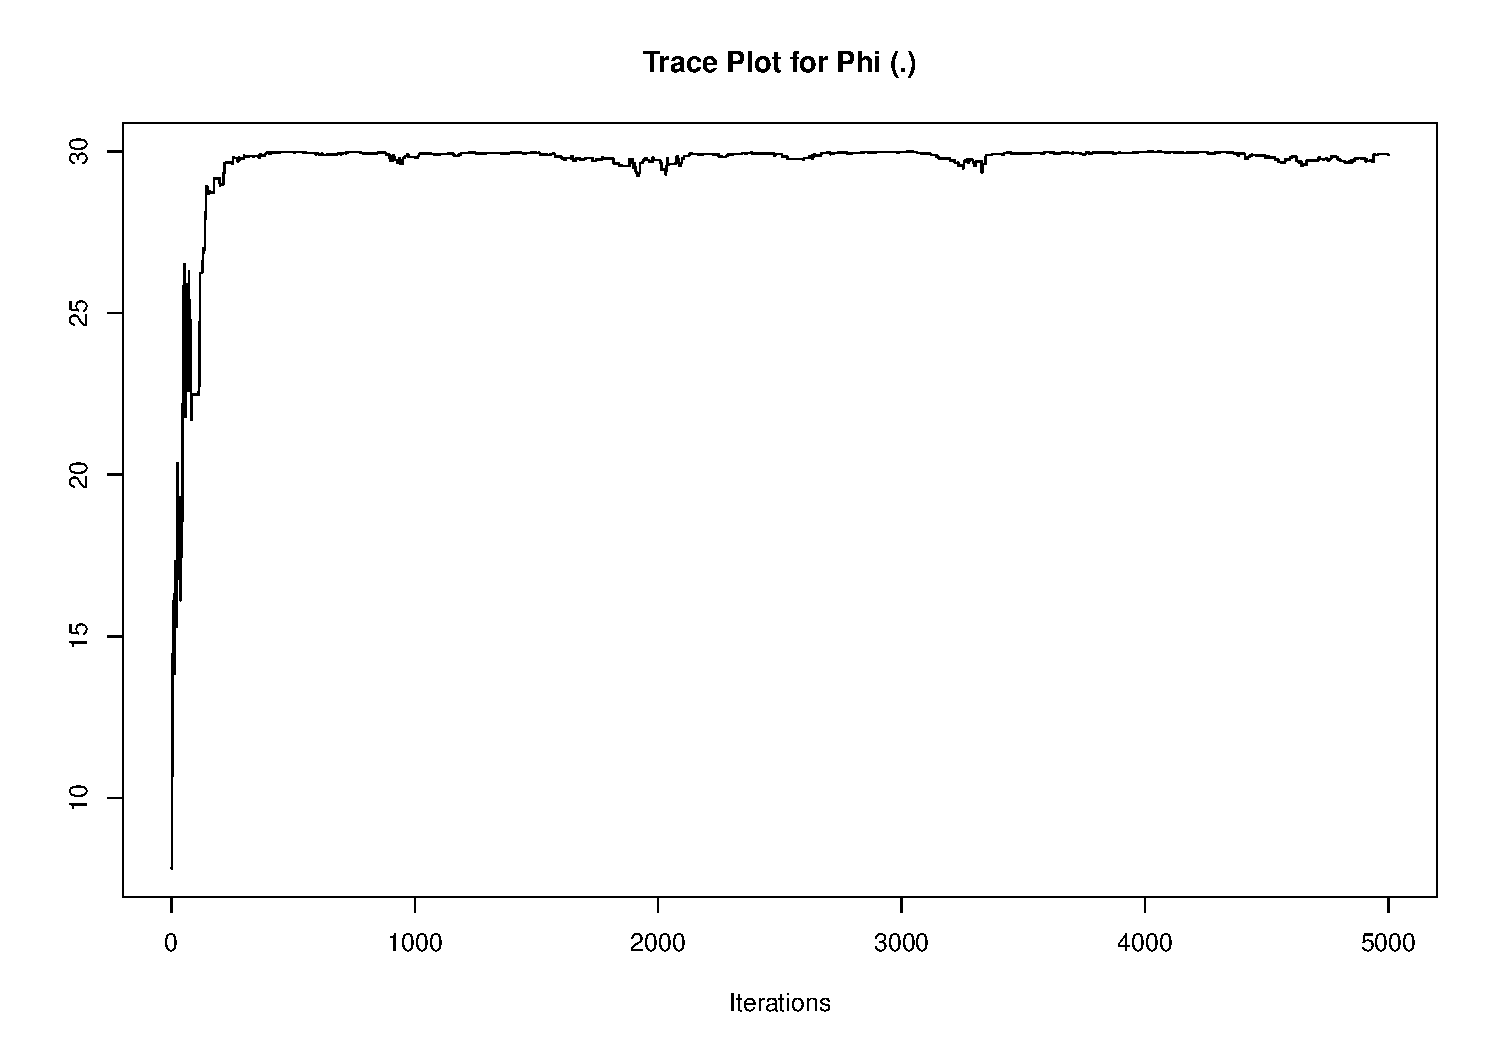
\includegraphics[keepaspectratio]{gc_files/figure-beamer/unnamed-chunk-30-1.pdf}}
\end{block}
\end{frame}

\begin{frame}{Bayesian Regression}
\phantomsection\label{bayesian-regression-6}
\begin{block}{MCMC Results - Trace Plot of Spatial Process Parameters -
σ²}
\phantomsection\label{mcmc-results---trace-plot-of-spatial-process-parameters---ux3c3uxb2}
\pandocbounded{\includegraphics[keepaspectratio]{gc_files/figure-beamer/unnamed-chunk-31-1.pdf}}
\end{block}
\end{frame}

\begin{frame}{Bayesian Regression}
\phantomsection\label{bayesian-regression-7}
\begin{block}{MCMC Results - Trace Plot of Spatial Process Parameters -
τ²}
\phantomsection\label{mcmc-results---trace-plot-of-spatial-process-parameters---ux3c4uxb2}
\pandocbounded{\includegraphics[keepaspectratio]{gc_files/figure-beamer/unnamed-chunk-32-1.pdf}}
\end{block}
\end{frame}

\begin{frame}{Bayesian Regression}
\phantomsection\label{bayesian-regression-8}
\begin{block}{Analysis of Trace Plots}
\phantomsection\label{analysis-of-trace-plots}
The trace plots for key spatial process parameters (Φ, σ², τ²) flatten
out after around 300 iterations. This indicates that the MCMC chain has
likely converged to the posterior distribution after the initial burn-in
period. The first 300 iterations are considered burn-in, and the
subsequent iterations reflect the true posterior. Additionally, the
chains exhibit no trends or systematic movements, suggesting effective
exploration of the parameter space.
\end{block}
\end{frame}

\begin{frame}{Bayesian Regression}
\phantomsection\label{bayesian-regression-9}
\begin{block}{MCMC Results - Autocorrelation of Spatial Process
Parameter - Φ}
\phantomsection\label{mcmc-results---autocorrelation-of-spatial-process-parameter---ux3c6}
\pandocbounded{\includegraphics[keepaspectratio]{gc_files/figure-beamer/unnamed-chunk-33-1.pdf}}
\end{block}
\end{frame}

\begin{frame}{Bayesian Regression}
\phantomsection\label{bayesian-regression-10}
\begin{block}{MCMC Results - Autocorrelation of Spatial Process
Parameter - σ²}
\phantomsection\label{mcmc-results---autocorrelation-of-spatial-process-parameter---ux3c3uxb2}
\pandocbounded{\includegraphics[keepaspectratio]{gc_files/figure-beamer/unnamed-chunk-34-1.pdf}}
\end{block}
\end{frame}

\begin{frame}{Bayesian Regression}
\phantomsection\label{bayesian-regression-11}
\begin{block}{MCMC Results - Autocorrelation of Spatial Process
Parameter - τ²}
\phantomsection\label{mcmc-results---autocorrelation-of-spatial-process-parameter---ux3c4uxb2}
\pandocbounded{\includegraphics[keepaspectratio]{gc_files/figure-beamer/unnamed-chunk-35-1.pdf}}
\end{block}
\end{frame}

\begin{frame}{Bayesian Regression}
\phantomsection\label{bayesian-regression-12}
\begin{block}{Analysis of Autocorrelation Plots}
\phantomsection\label{analysis-of-autocorrelation-plots}
The autocorrelation plots for Φ and σ² show similar trends, with both
parameters exhibiting a slow decay in autocorrelation, indicating
moderate dependence between successive samples. This suggests reasonable
mixing for these parameters. However, for τ², the autocorrelation decays
to a lower value of 0.25, indicating slower mixing and stronger
dependence between samples. This slower decay for τ² suggests the chain
may be struggling to effectively explore the parameter space for this
parameter, potentially due to strong correlations with other parameters
or insufficient mixing.
\end{block}
\end{frame}

\section{Group Challenge 3}\label{group-challenge-3}

\begin{frame}{Jittering}
\phantomsection\label{jittering}
Formal Jittering. We set for 0.03 as standard deviation.

\pandocbounded{\includegraphics[keepaspectratio]{gc_files/figure-beamer/map-1.pdf}}
\end{frame}

\begin{frame}[fragile]{Regression}
\phantomsection\label{regression}
We run a linear model with the 4 covariates for future initial
parameters setting.

\begin{verbatim}

Call:
lm(formula = y ~ ., data = X_selected_df)

Residuals:
    Min      1Q  Median      3Q     Max 
-2342.4  -457.1    12.6   467.6  3239.3 

Coefficients:
                           Estimate Std. Error t value Pr(>|t|)    
(Intercept)              2563.37373  114.97376  22.295  < 2e-16 ***
birth_weight_type_recall   89.92422   71.37700   1.260 0.207848    
mother_bmi                  0.16857    0.03512   4.800 1.69e-06 ***
sex_of_child_male         106.70534   28.71063   3.717 0.000207 ***
mother_current_age         -4.52190    2.74553  -1.647 0.099689 .  
---
Signif. codes:  0 '***' 0.001 '**' 0.01 '*' 0.05 '.' 0.1 ' ' 1

Residual standard error: 698.4 on 2378 degrees of freedom
Multiple R-squared:  0.01605,   Adjusted R-squared:  0.01439 
F-statistic: 9.695 on 4 and 2378 DF,  p-value: 8.905e-08
\end{verbatim}

\begin{verbatim}
B₀: 89.924, B1: 0.169, B2: 106.705, B3: -4.522
\end{verbatim}
\end{frame}

\begin{frame}{MGP Fitting}
\phantomsection\label{mgp-fitting}
\end{frame}

\begin{frame}{MGP Trace and Density Plots for Regression Coefficients
(β1)}
\phantomsection\label{mgp-trace-and-density-plots-for-regression-coefficients-ux3b21}
\pandocbounded{\includegraphics[keepaspectratio]{gc_files/figure-beamer/plot-1.pdf}}
\end{frame}

\begin{frame}{MGP Trace and Density Plots for Regression Coefficients
(β2)}
\phantomsection\label{mgp-trace-and-density-plots-for-regression-coefficients-ux3b22}
\pandocbounded{\includegraphics[keepaspectratio]{gc_files/figure-beamer/unnamed-chunk-36-1.pdf}}
\end{frame}

\begin{frame}{MGP Trace and Density Plots for Regression Coefficients
(β3)}
\phantomsection\label{mgp-trace-and-density-plots-for-regression-coefficients-ux3b23}
\pandocbounded{\includegraphics[keepaspectratio]{gc_files/figure-beamer/unnamed-chunk-37-1.pdf}}
\end{frame}

\begin{frame}{MGP Trace and Density Plots for Regression Coefficients
(β4)}
\phantomsection\label{mgp-trace-and-density-plots-for-regression-coefficients-ux3b24}
\pandocbounded{\includegraphics[keepaspectratio]{gc_files/figure-beamer/unnamed-chunk-38-1.pdf}}
\end{frame}

\begin{frame}{MGP Trace and Density Plots for Hyperparameters (τ²)}
\phantomsection\label{mgp-trace-and-density-plots-for-hyperparameters-ux3c4uxb2}
\pandocbounded{\includegraphics[keepaspectratio]{gc_files/figure-beamer/unnamed-chunk-39-1.pdf}}
\end{frame}

\begin{frame}{MGP Trace and Density Plots for Hyperparameters (φ)}
\phantomsection\label{mgp-trace-and-density-plots-for-hyperparameters-ux3c6}
\pandocbounded{\includegraphics[keepaspectratio]{gc_files/figure-beamer/unnamed-chunk-40-1.pdf}}
\end{frame}

\begin{frame}{MGP Trace and Density Plots for Hyperparameters (σ²)}
\phantomsection\label{mgp-trace-and-density-plots-for-hyperparameters-ux3c3uxb2}
\pandocbounded{\includegraphics[keepaspectratio]{gc_files/figure-beamer/unnamed-chunk-41-1.pdf}}
\end{frame}

\begin{frame}{MGP Trace and Density Plots - Analysis}
\phantomsection\label{mgp-trace-and-density-plots---analysis}
The convergence is reached after approximately 6,000 iterations, so we
ran for 28,000 iterations and burn the first 8,000. We initialize the
regression coefficients (\(\beta\)) from the linear regression with the
covariates we are interested in.
\end{frame}

\begin{frame}{Posterior Predictive Map}
\phantomsection\label{posterior-predictive-map}
\pandocbounded{\includegraphics[keepaspectratio]{gc_files/figure-beamer/prediction-1.pdf}}
\end{frame}

\begin{frame}{Empirical Spatial Variogram}
\phantomsection\label{empirical-spatial-variogram}
\pandocbounded{\includegraphics[keepaspectratio]{gc_files/figure-beamer/variogram-1.pdf}}
\end{frame}

\begin{frame}[fragile]{Nonspatial Linear Regression}
\phantomsection\label{nonspatial-linear-regression}
\begin{verbatim}

Call:
lm(formula = birth_weight ~ birth_weight_type + mother_bmi + 
    sex_of_child + mother_current_age, data = reg_data)

Residuals:
    Min      1Q  Median      3Q     Max 
-2342.4  -457.1    12.6   467.6  3239.3 

Coefficients:
                                Estimate Std. Error t value Pr(>|t|)    
(Intercept)                   2653.29795   90.88762  29.193  < 2e-16 ***
birth_weight_typewritten card  -89.92422   71.37700  -1.260 0.207848    
mother_bmi                       0.16857    0.03512   4.800 1.69e-06 ***
sex_of_childmale               106.70534   28.71063   3.717 0.000207 ***
mother_current_age              -4.52190    2.74553  -1.647 0.099689 .  
---
Signif. codes:  0 '***' 0.001 '**' 0.01 '*' 0.05 '.' 0.1 ' ' 1

Residual standard error: 698.4 on 2378 degrees of freedom
Multiple R-squared:  0.01605,   Adjusted R-squared:  0.01439 
F-statistic: 9.695 on 4 and 2378 DF,  p-value: 8.905e-08
\end{verbatim}
\end{frame}

\begin{frame}[fragile]{Spatial Nearest Neighbor Gaussian Process}
\phantomsection\label{spatial-nearest-neighbor-gaussian-process}
\begin{verbatim}
----------------------------------------
    Building the neighbor list
----------------------------------------
\end{verbatim}

\begin{verbatim}
----------------------------------------
Building the neighbors of neighbors list
----------------------------------------
\end{verbatim}

\begin{verbatim}
----------------------------------------
    Model description
----------------------------------------
NNGP Latent model fit with 2383 observations.

Number of covariates 5 (including intercept if specified).

Using the exponential spatial correlation model.

Using 15 nearest neighbors.

Number of MCMC samples 2000.

Priors and hyperpriors:
    beta flat.
    sigma.sq IG hyperpriors shape=2.00000 and scale=1.00000
    tau.sq IG hyperpriors shape=2.00000 and scale=1.00000
    phi Unif hyperpriors a=3.00000 and b=30.00000


Source not compiled with OpenMP support.
----------------------------------------
        Sampling
----------------------------------------
Sampled: 100 of 2000, 5.00%
Report interval Metrop. Acceptance rate: 57.00%
Overall Metrop. Acceptance rate: 57.00%
-------------------------------------------------
Sampled: 200 of 2000, 10.00%
Report interval Metrop. Acceptance rate: 81.00%
Overall Metrop. Acceptance rate: 69.00%
-------------------------------------------------
Sampled: 300 of 2000, 15.00%
Report interval Metrop. Acceptance rate: 66.00%
Overall Metrop. Acceptance rate: 68.00%
-------------------------------------------------
Sampled: 400 of 2000, 20.00%
Report interval Metrop. Acceptance rate: 77.00%
Overall Metrop. Acceptance rate: 70.25%
-------------------------------------------------
Sampled: 500 of 2000, 25.00%
Report interval Metrop. Acceptance rate: 63.00%
Overall Metrop. Acceptance rate: 68.80%
-------------------------------------------------
Sampled: 600 of 2000, 30.00%
Report interval Metrop. Acceptance rate: 72.00%
Overall Metrop. Acceptance rate: 69.33%
-------------------------------------------------
Sampled: 700 of 2000, 35.00%
Report interval Metrop. Acceptance rate: 87.00%
Overall Metrop. Acceptance rate: 71.86%
-------------------------------------------------
Sampled: 800 of 2000, 40.00%
Report interval Metrop. Acceptance rate: 69.00%
Overall Metrop. Acceptance rate: 71.50%
-------------------------------------------------
Sampled: 900 of 2000, 45.00%
Report interval Metrop. Acceptance rate: 65.00%
Overall Metrop. Acceptance rate: 70.78%
-------------------------------------------------
Sampled: 1000 of 2000, 50.00%
Report interval Metrop. Acceptance rate: 67.00%
Overall Metrop. Acceptance rate: 70.40%
-------------------------------------------------
Sampled: 1100 of 2000, 55.00%
Report interval Metrop. Acceptance rate: 59.00%
Overall Metrop. Acceptance rate: 69.36%
-------------------------------------------------
Sampled: 1200 of 2000, 60.00%
Report interval Metrop. Acceptance rate: 42.00%
Overall Metrop. Acceptance rate: 67.08%
-------------------------------------------------
Sampled: 1300 of 2000, 65.00%
Report interval Metrop. Acceptance rate: 48.00%
Overall Metrop. Acceptance rate: 65.62%
-------------------------------------------------
Sampled: 1400 of 2000, 70.00%
Report interval Metrop. Acceptance rate: 60.00%
Overall Metrop. Acceptance rate: 65.21%
-------------------------------------------------
Sampled: 1500 of 2000, 75.00%
Report interval Metrop. Acceptance rate: 65.00%
Overall Metrop. Acceptance rate: 65.20%
-------------------------------------------------
Sampled: 1600 of 2000, 80.00%
Report interval Metrop. Acceptance rate: 60.00%
Overall Metrop. Acceptance rate: 64.88%
-------------------------------------------------
Sampled: 1700 of 2000, 85.00%
Report interval Metrop. Acceptance rate: 74.00%
Overall Metrop. Acceptance rate: 65.41%
-------------------------------------------------
Sampled: 1800 of 2000, 90.00%
Report interval Metrop. Acceptance rate: 73.00%
Overall Metrop. Acceptance rate: 65.83%
-------------------------------------------------
Sampled: 1900 of 2000, 95.00%
Report interval Metrop. Acceptance rate: 78.00%
Overall Metrop. Acceptance rate: 66.47%
-------------------------------------------------
Sampled: 2000 of 2000, 100.00%
Report interval Metrop. Acceptance rate: 62.00%
Overall Metrop. Acceptance rate: 66.25%
-------------------------------------------------
\end{verbatim}

\begin{verbatim}

Call:
spNNGP(formula = birth_weight ~ birth_weight_type + mother_bmi + 
    sex_of_child + mother_current_age, data = reg_data, coords = coords, 
    method = "latent", n.neighbors = 15, starting = starting, 
    tuning = tuning, priors = priors, cov.model = cov.model, 
    n.samples = n.samples, n.omp.threads = 4, return.neighbor.info = TRUE, 
    fit.rep = TRUE, sub.sample = list(start = burn_in + 1, thin = thin_val))

Model class is NNGP, method latent, family gaussian.

Model object contains 2000 MCMC samples.

Chain sub.sample:
start = 1000
end = 2000
thin = 1
samples size = 1001
                              2.5%        25%         50%         75%        
(Intercept)                   2465.8234   2589.3557   2652.2175   2711.6499  
birth_weight_typewritten card -222.6849   -131.6917   -85.9321    -39.8576   
mother_bmi                    0.1038      0.1462      0.1713      0.1936     
sex_of_childmale              52.8149     87.5137     107.4503    126.9807   
mother_current_age            -9.7638     -6.4262     -4.4589     -2.6049    
sigma.sq                      186.6622    210.1165    227.7529    256.8892   
tau.sq                        460974.9390 477274.3627 486555.3655 497041.3538
phi                           17.3649     20.2631     22.5814     25.0871    
                              97.5%      
(Intercept)                   2818.3560  
birth_weight_typewritten card 45.7286    
mother_bmi                    0.2402     
sex_of_childmale              163.6529   
mother_current_age            0.5645     
sigma.sq                      326.3804   
tau.sq                        513818.2239
phi                           27.7145    
\end{verbatim}
\end{frame}

\begin{frame}{NNGP Trace and Density Plots for Regression Coefficients
(β1)}
\phantomsection\label{nngp-trace-and-density-plots-for-regression-coefficients-ux3b21}
\pandocbounded{\includegraphics[keepaspectratio]{gc_files/figure-beamer/unnamed-chunk-45-1.pdf}}
\end{frame}

\begin{frame}{NNGP Trace and Density Plots for Regression Coefficients
(β2)}
\phantomsection\label{nngp-trace-and-density-plots-for-regression-coefficients-ux3b22}
\pandocbounded{\includegraphics[keepaspectratio]{gc_files/figure-beamer/unnamed-chunk-46-1.pdf}}
\end{frame}

\begin{frame}{NNGP Trace and Density Plots for Regression Coefficients
(β3)}
\phantomsection\label{nngp-trace-and-density-plots-for-regression-coefficients-ux3b23}
\pandocbounded{\includegraphics[keepaspectratio]{gc_files/figure-beamer/unnamed-chunk-47-1.pdf}}
\end{frame}

\begin{frame}{NNGP Trace and Density Plots for Regression Coefficients
(β4)}
\phantomsection\label{nngp-trace-and-density-plots-for-regression-coefficients-ux3b24}
\pandocbounded{\includegraphics[keepaspectratio]{gc_files/figure-beamer/unnamed-chunk-48-1.pdf}}
\end{frame}

\begin{frame}{NNGP Trace and Density Plots for Regression Coefficients
(β5)}
\phantomsection\label{nngp-trace-and-density-plots-for-regression-coefficients-ux3b25}
\pandocbounded{\includegraphics[keepaspectratio]{gc_files/figure-beamer/unnamed-chunk-49-1.pdf}}
\end{frame}

\begin{frame}{NNGP Trace and Density Plots for Regression Coefficients
(β) - Analysis}
\phantomsection\label{nngp-trace-and-density-plots-for-regression-coefficients-ux3b2---analysis}
The trace plots for the \(\beta\) parameters illustrate that after an
initial burn-in period the chains stabilize and fluctuate around a fixed
mean, indicating good mixing and convergence. Corresponding density
plots show smooth, unimodal distributions for each coefficient, which
suggests that the posterior estimates for the fixed effects are reliable
\end{frame}

\begin{frame}{NNGP Trace and Density Plots for Hyperparameters (φ)}
\phantomsection\label{nngp-trace-and-density-plots-for-hyperparameters-ux3c6}
\pandocbounded{\includegraphics[keepaspectratio]{gc_files/figure-beamer/unnamed-chunk-50-1.pdf}}
\end{frame}

\begin{frame}{NNGP Trace and Density Plots for Hyperparameters (σ²)}
\phantomsection\label{nngp-trace-and-density-plots-for-hyperparameters-ux3c3uxb2}
\pandocbounded{\includegraphics[keepaspectratio]{gc_files/figure-beamer/unnamed-chunk-51-1.pdf}}
\end{frame}

\begin{frame}{NNGP Trace and Density Plots for Hyperparameters (τ²)}
\phantomsection\label{nngp-trace-and-density-plots-for-hyperparameters-ux3c4uxb2}
\pandocbounded{\includegraphics[keepaspectratio]{gc_files/figure-beamer/unnamed-chunk-52-1.pdf}}
\end{frame}

\begin{frame}{NNGP Trace and Density Plots for Hyperparameters -
Analysis}
\phantomsection\label{nngp-trace-and-density-plots-for-hyperparameters---analysis}
For the spatial decay parameter (φ) and variance components (σ² for the
spatial process and τ² for the nugget), the trace plots demonstrate that
the chains converge after a burn-in period. The density plots reveal
that although φ exhibits some right skew (with a long tail), all
hyperparameters exhibit unimodal posterior distributions. This indicates
that the model has successfully explored the parameter space and reached
a stable posterior distribution.
\end{frame}

\begin{frame}{Trace and Density Plots for Selected Latent Spatial
Effects (w(1131))}
\phantomsection\label{trace-and-density-plots-for-selected-latent-spatial-effects-w1131}
\pandocbounded{\includegraphics[keepaspectratio]{gc_files/figure-beamer/unnamed-chunk-53-1.pdf}}
\end{frame}

\begin{frame}{Trace and Density Plots for Selected Latent Spatial
Effects (w(397))}
\phantomsection\label{trace-and-density-plots-for-selected-latent-spatial-effects-w397}
\pandocbounded{\includegraphics[keepaspectratio]{gc_files/figure-beamer/unnamed-chunk-54-1.pdf}}
\end{frame}

\begin{frame}{Trace and Density Plots for Selected Latent Spatial
Effects (w(318))}
\phantomsection\label{trace-and-density-plots-for-selected-latent-spatial-effects-w318}
\pandocbounded{\includegraphics[keepaspectratio]{gc_files/figure-beamer/unnamed-chunk-55-1.pdf}}
\end{frame}

\begin{frame}{Trace and Density Plots for Selected Latent Spatial
Effects (w(266))}
\phantomsection\label{trace-and-density-plots-for-selected-latent-spatial-effects-w266}
\pandocbounded{\includegraphics[keepaspectratio]{gc_files/figure-beamer/unnamed-chunk-56-1.pdf}}
\end{frame}

\begin{frame}{Trace and Density Plots for Selected Latent Spatial
Effects (w(1354))}
\phantomsection\label{trace-and-density-plots-for-selected-latent-spatial-effects-w1354}
\pandocbounded{\includegraphics[keepaspectratio]{gc_files/figure-beamer/unnamed-chunk-57-1.pdf}}
\end{frame}

\begin{frame}{Trace and Density Plots for Selected Latent Spatial
Effects - Analysis}
\phantomsection\label{trace-and-density-plots-for-selected-latent-spatial-effects---analysis}
The trace plots for the latent spatial effect w(s) at selected locations
show stable fluctuations over the MCMC iterations, with no evident
trends or abrupt jumps, which confirms convergence. Their density plots,
while showing some variability across locations, are generally smooth
and unimodal. This implies that the spatial random effects are
well‐estimated at the individual locations.
\end{frame}

\begin{frame}{Posterior Predictive Map at Observed Locations}
\phantomsection\label{posterior-predictive-map-at-observed-locations}
\pandocbounded{\includegraphics[keepaspectratio]{gc_files/figure-beamer/unnamed-chunk-59-1.pdf}}
\end{frame}

\begin{frame}{Posterior Predictive Map at Observed Locations}
\phantomsection\label{posterior-predictive-map-at-observed-locations-1}
This map displays the posterior predictive distribution for the observed
locations, derived from one selected draw (or the posterior mean) of the
y\_rep samples. The color scale represents the predicted birth weight
values. The relatively uniform distribution of colors (without
large-scale gradients) suggests that the NNGP model has effectively
accounted for spatial variation in the observed response
\end{frame}

\begin{frame}{Empirical Variogram of Posterior Predictive Values}
\phantomsection\label{empirical-variogram-of-posterior-predictive-values}
\pandocbounded{\includegraphics[keepaspectratio]{gc_files/figure-beamer/unnamed-chunk-60-1.pdf}}
\end{frame}

\begin{frame}{Residuals Variogram of Posterior Predictive Values}
\phantomsection\label{residuals-variogram-of-posterior-predictive-values}
\pandocbounded{\includegraphics[keepaspectratio]{gc_files/figure-beamer/unnamed-chunk-61-1.pdf}}
\end{frame}

\begin{frame}{Residuals Variogram of Posterior Predictive Values}
\phantomsection\label{residuals-variogram-of-posterior-predictive-values-1}
The variogram of the model residuals displays a moderate increase at
medium distances before leveling off. This pattern indicates that while
most of the spatial dependence has been accounted for by the model, some
minor spatial correlation remains among nearby observations. However,
the overall level of semivariance does not continue to increase with
distance, which supports the conclusion that the residual spatial
autocorrelation is weak and likely due to random variability rather than
a systematic bias. We see the sharp drop of semivariance when distance
is greater than 200, this is due to the limited data at large distance.
\end{frame}

\begin{frame}{Estimated Latent Process w(s)}
\phantomsection\label{estimated-latent-process-ws}
\pandocbounded{\includegraphics[keepaspectratio]{gc_files/figure-beamer/unnamed-chunk-62-1.pdf}}
\end{frame}

\begin{frame}{Estimated Latent Process w(s)}
\phantomsection\label{estimated-latent-process-ws-1}
The map clearly illustrates the spatial heterogeneity in the latent
field, highlighting areas where the model detects higher or lower
spatial effects. This visualization helps in interpreting the spatial
structure that the NNGP model has captured beyond what is explained by
the covariates.
\end{frame}

\begin{frame}{Empirical Variogram of the Estimated Latent Process w(s)}
\phantomsection\label{empirical-variogram-of-the-estimated-latent-process-ws}
\pandocbounded{\includegraphics[keepaspectratio]{gc_files/figure-beamer/unnamed-chunk-63-1.pdf}}
\end{frame}

\begin{frame}{Empirical Variogram of the Estimated Latent Process w(s)}
\phantomsection\label{empirical-variogram-of-the-estimated-latent-process-ws-1}
The latent spatial process w(s) exhibits some small-scale variability
near neighboring locations, causing the semivariance to be unexpectedly
high at very short lags. As distance increases, the semivariance
declines and fluctuates, indicating that the spatial correlation in w(s)
is relatively short-ranged.
\end{frame}




\end{document}
